\section[中心力场的一般概念]{中心力场的一般概念} \label{sec:05.01} % 
% \makebox[5em][s]{} % 短题目拉间距

质量为$\mu$的粒子在中心力场中运动(暂不考虑粒子的自旋),能量算符可以表示成
\begin{empheq}{equation}\label{eq51.1}
	\hat{H}=\frac{\hat{\boldsymbol{p}}^{2}}{2\mu}+V(r)=-\frac{\hbar^{2}}{2\mu}\nabla^{2}+V(r)
\end{empheq}
$V(r)$为势能粒子受到的作用力为
\begin{empheq}{equation}\label{eq51.2}
	\boldsymbol{F}=-\nabla V=-\frac{dV}{dr}\frac{\boldsymbol{r}}{r}
\end{empheq}
由于力矩$\boldsymbol{r}\times\boldsymbol{F}$恒等于0,所以轨道角动量$\boldsymbol{L}=\boldsymbol{r}\times\boldsymbol{p}$是守恒量.由于$\hat{H}$是偶宇称,所以宇称守恒.此外,根据$V(r)$的特殊性质,还可能存在其他守恒量.

通常,取$(\hat{H},\hat{\boldsymbol{L}}^{2},\hat{L}_{z})$作为守恒量完全集,以它们的共同本征函数作为基本的能量本征函数(能量表象的基矢),用以处理与中心力场有关的各种问题.

{\heiti 1. 球谐函数}

在球坐标$(r,\theta,\varphi)$中,$\hat{\boldsymbol{L}}^{2},\hat{L}_{z}$的算符表示为(见附录\ref{A03})
\eqlong
\begin{empheq}{align}	%3,4
	\hat{\boldsymbol{L}}^{2}=-\hbar^{2}\bigg(\frac{1}{\sin\theta}&\frac{\partial}{\partial\theta}\sin\theta\frac{\partial}{\partial\theta}+\frac{1}{\sin^{2}\theta}\frac{\partial^{2}}{\partial\varphi^{2}}\bigg)		\label{eq51.3}\\
	\hat{L}_{z}&=-i\hbar\frac{\partial}{\partial\varphi}		\label{eq51.4}
\end{empheq}\eqnormal
按照角动量的一般理论($\S$\ref{sec:04.07}),它们的本征值是
\begin{empheq}{align}\label{eq51.5}
	\boldsymbol{L}^{2} &=l(l+1)\hbar^{2},\quad l=0,1,2,\cdots	\nonumber\\
	L_{z}&=m\hbar,\quad m=0,\pm1,\pm2,\cdots,\pm l
\end{empheq}
$\hat{\boldsymbol{L}}^{2},\hat{L}_{z}$的共同本征函数习惯上记成$Y_{lm}(\theta,\varphi)$,满足本征方程
\begin{subequations}
	\begin{empheq}{align}
		\hat{\boldsymbol{L}}^{2}Y_{lm}&=l(l+1)\hbar^{2}Y_{lm}	\label{eq51.6a}\\
		\hat{L}_{z}Y_{lm}&=m\hbar Y_{lm}	\label{eq51.6b}
	\end{empheq}
\end{subequations}
$Y_{lm}(\theta,\varphi)$称为球谐函数,其具体函数形式(见附录\ref{A04})为
\eqlong
\begin{empheq}{equation}\label{eq51.7}
	Y_{lm}(\theta,\varphi)=(-1)^{m}\bigg[\frac{2l+1}{4\pi}\frac{(l-m)!}{(l+m)!}\bigg]^{\frac{1}{2}}P_{l}^{m}(\cos\theta)e^{im\varphi}
\end{empheq}\eqnormal
其中$P_{l}^{m}$是连带勒让德函数.

{\heiti 2. 径向方程}

拉普拉斯算符$\nabla^{2}$的球坐标表示式是
\eqllong
\begin{empheq}{equation}\label{eq51.8}
	\nabla^{2}=\frac{1}{r^{2}}\frac{\partial}{\partial r}r^{2}\frac{\partial}{\partial r}+\frac{1}{r^{2}}\bigg(\frac{1}{\sin\theta}\frac{\partial}{\partial \theta}\sin\theta\frac{\partial}{\partial \theta}+\frac{1}{\sin^{2}\theta}\frac{\partial^{2}}{\partial \varphi^{2}}\bigg)
\end{empheq}\eqnormal
因此,总能量算符可以表示成
\eqlong
\begin{empheq}{equation}\label{eq51.9}
	\hat{H}=-\frac{\hbar^{2}}{2\mu}\frac{1}{r^{2}}\frac{\partial}{\partial r}r^{2}\frac{\partial}{\partial r}+\frac{1}{2\mu r}\hat{\boldsymbol{L}}^{2}+V(r)
\end{empheq}\eqnormal
习惯上常称第一项为径向动能算符,第二项为离心势能算符,实际上它也是动能(算符)的一部分.

$\hat{H},\hat{\boldsymbol{L}}^{2},\hat{L}_{z}$的共同本征函数显然可以表示成
\begin{empheq}{equation}\label{eq51.10}
	\varPsi(r,\theta,\varphi)=R(r)Y_{lm}(\theta,\varphi)
\end{empheq}
其中球谐函数$Y_{lm}$保证$\varPsi$是$\hat{\boldsymbol{L}}^{2}$和$\hat{L}_{z}$上的本征函数,$R(r)$称为径向波函数.$\varPsi$应该满足能量本征方程
\eqshort
\begin{empheq}{equation}\label{eq51.11}
	\hat{H}\varPsi=E\varPsi
\end{empheq}\eqnormal
将\eqref{eq51.9}、\eqref{eq51.10}式代入\eqref{eq51.11}式,得到$R(r)$满足的方程
\eqllong
\begin{empheq}{equation}\label{eq51.12}
	\bigg[-\frac{\hbar^{2}}{2\mu}\frac{1}{r^{2}}\frac{d}{dr}r^{2}\frac{d}{dr}+\frac{l(l+1)\hbar^{2}}{2\mu r^{2}}+V(r)\bigg]R(r)=ER(r)
\end{empheq}\eqnormal
称为径向方程.能量$E$的本征值以及$R(r)$的函数形式应该求解上式而决定.

\noindent 由于
\begin{empheq}{equation*}
	\frac{1}{r^{2}}\frac{d}{dr}r^{2}R(r)\equiv\frac{1}{r}\frac{d^{2}}{dr^{2}}[rR(r)]
\end{empheq}
所以通常令
\begin{empheq}{equation}\label{eq51.13}
	u(r)=rR(r)
\end{empheq}
而\eqref{eq51.12}式简化成
\eqlong
\begin{empheq}{equation}\label{eq51.14}
	\bigg[-\frac{\hbar^{2}}{2\mu}\frac{d^{2}}{dr^{2}}+\frac{l(l+1)\hbar^{2}}{2\mu r^{2}}+V(r)\bigg]u(r)=Eu(r)
\end{empheq}\eqnormal
上式也称为径向方程,它形式上很像一维定态薛定谔方程,只是真正的势能$V(r)$换成了等效势能
\begin{empheq}{equation}\label{eq51.15}
	V_{l}(r)=V(r)+\frac{l(l+1)\hbar^{2}}{2\mu r^{2}}
\end{empheq}
其中第二项是离心势能.

径向波函数$R(r)$或$u(r)$除了满足径向方程外,还必须满足某些边界条件.束缚态波函数满足归一化条件
\begin{empheq}{equation}\label{eq51.16}
	\int_{\text{全}}\varPsi^{*}\varPsi d\tau=1
\end{empheq}
亦即
\begin{empheq}{equation*}\label{eq51.16'}
	\int_{0}^{\infty}|R(r)|^{2}r^{2}dr=\int_{0}^{\infty}|u(r)|^{2}dr=1
	\tag{$5.1.16^{\prime}$}
\end{empheq}

在力心$(r=0)$附近波函数的性质对于许多问题都是重要的.如果$r\rightarrow 0$处势能$V(r)$是解析的,或者$V(r)$以下列方式趋于无限,
\begin{empheq}{equation}\label{eq51.17}
	r\rightarrow 0,\quad V(r)\propto r^{-s},\quad 0<s<2
\end{empheq}
则由\eqref{eq51.14}式,在$r\sim 0$附近,
\begin{empheq}{align*}
	\frac{d^{2}}{dr^{2}}u&\approx\frac{l(l+1)u}{r^{2}}	\\
	u&\approx r^{l+1},r^{-l}
\end{empheq}
为了满足归一化条件,必须取第一个解\footnote{$l=0$时,取$R\approx Cr^{-l-1}=Cr^{-1}$虽能满足归一化条件,但是不满足能量本征方程\eqref{eq51.11},因为这时$\varPsi\approx\frac{C}{\sqrt{4\pi}}\frac{1}{r},\nabla^{2}\varPsi\approx -\sqrt{4\pi}C\delta(\boldsymbol{r})$	\label{F.5-1} }
\begin{empheq}{align}	%18,19
	r\rightarrow 0,\quad u\approx Cr^{l+1},\quad R(r)\approx Cr^{l}		\label{eq51.18}\\
	\varPsi=R(r)Y_{lm}(\theta,\varphi)\approx Cr^{l}Y_{lm}(\theta,\varphi)		\label{eq51.19}
\end{empheq}
如$l\neq 0,r\rightarrow 0$处$\varPsi\rightarrow 0$,粒子在力心附近出现概率趋于0.

{\heiti 3. 能谱构造}

在许多问题中,$r\rightarrow\infty$处作用力$F\rightarrow 0$,这时通常取$V(r\rightarrow\infty)=0$,作为能量的标准.这种情况下,$r\rightarrow\infty$处\eqref{eq51.14}式简化成
\begin{empheq}{equation}\label{eq51.20}
	\frac{d^{2}}{dr^{2}}u+\frac{2\mu E}{\hbar^{2}}u\approx 0
\end{empheq}
如$E>0$,上式的解为
\eqlong
\begin{empheq}{equation}\label{eq51.21}
	u(r)\approx C_{1}\sin kr+C_{2}\cos kr,\quad k=\frac{\sqrt{2\mu E}}{\hbar}
\end{empheq}
不论$C_{1},C_{2}$取什么值,$u(r)$总是有限的,$k$及$E$可以不受限制,连续变化.渐近形式为\eqref{eq51.21}式的波函数,显然是不能满足归一化条件\eqref{eq51.16'}的,因此$E>0$相应于游离态,属于连续能谱.

如$E<0$,\eqref{eq51.20}式的解为
\begin{empheq}{equation}\label{eq51.22}
	u(r)\approx C_{3}e^{-\alpha r}+C_{4}e^{\alpha r},\quad \alpha=\frac{\sqrt{-2\mu E}}{\hbar}
\end{empheq}\eqnormal
为了满足归一化条件,必须$C_{4}=0$.在这个限制条件下,通常将导致能级的量子化.相应的波函数显然是平方可积的,可以归一化,因此是束缚态.

为了求出束缚态能级,需要解径向方程(12)或(14).一般说,对于每一个$l$值$(l=0,1,2,\cdots)$可以解出一组能级,由低到高依次记为$E_{1l},E_{2l},E_{3l},\cdots$.由于离心势能随$l$的升高而增大,所以各组能级的起点(即$E_{1l}$)亦随$l$的升高而升高,如图\ref{fig.5-1}所示
\begin{figure}[!h]
	\centering
	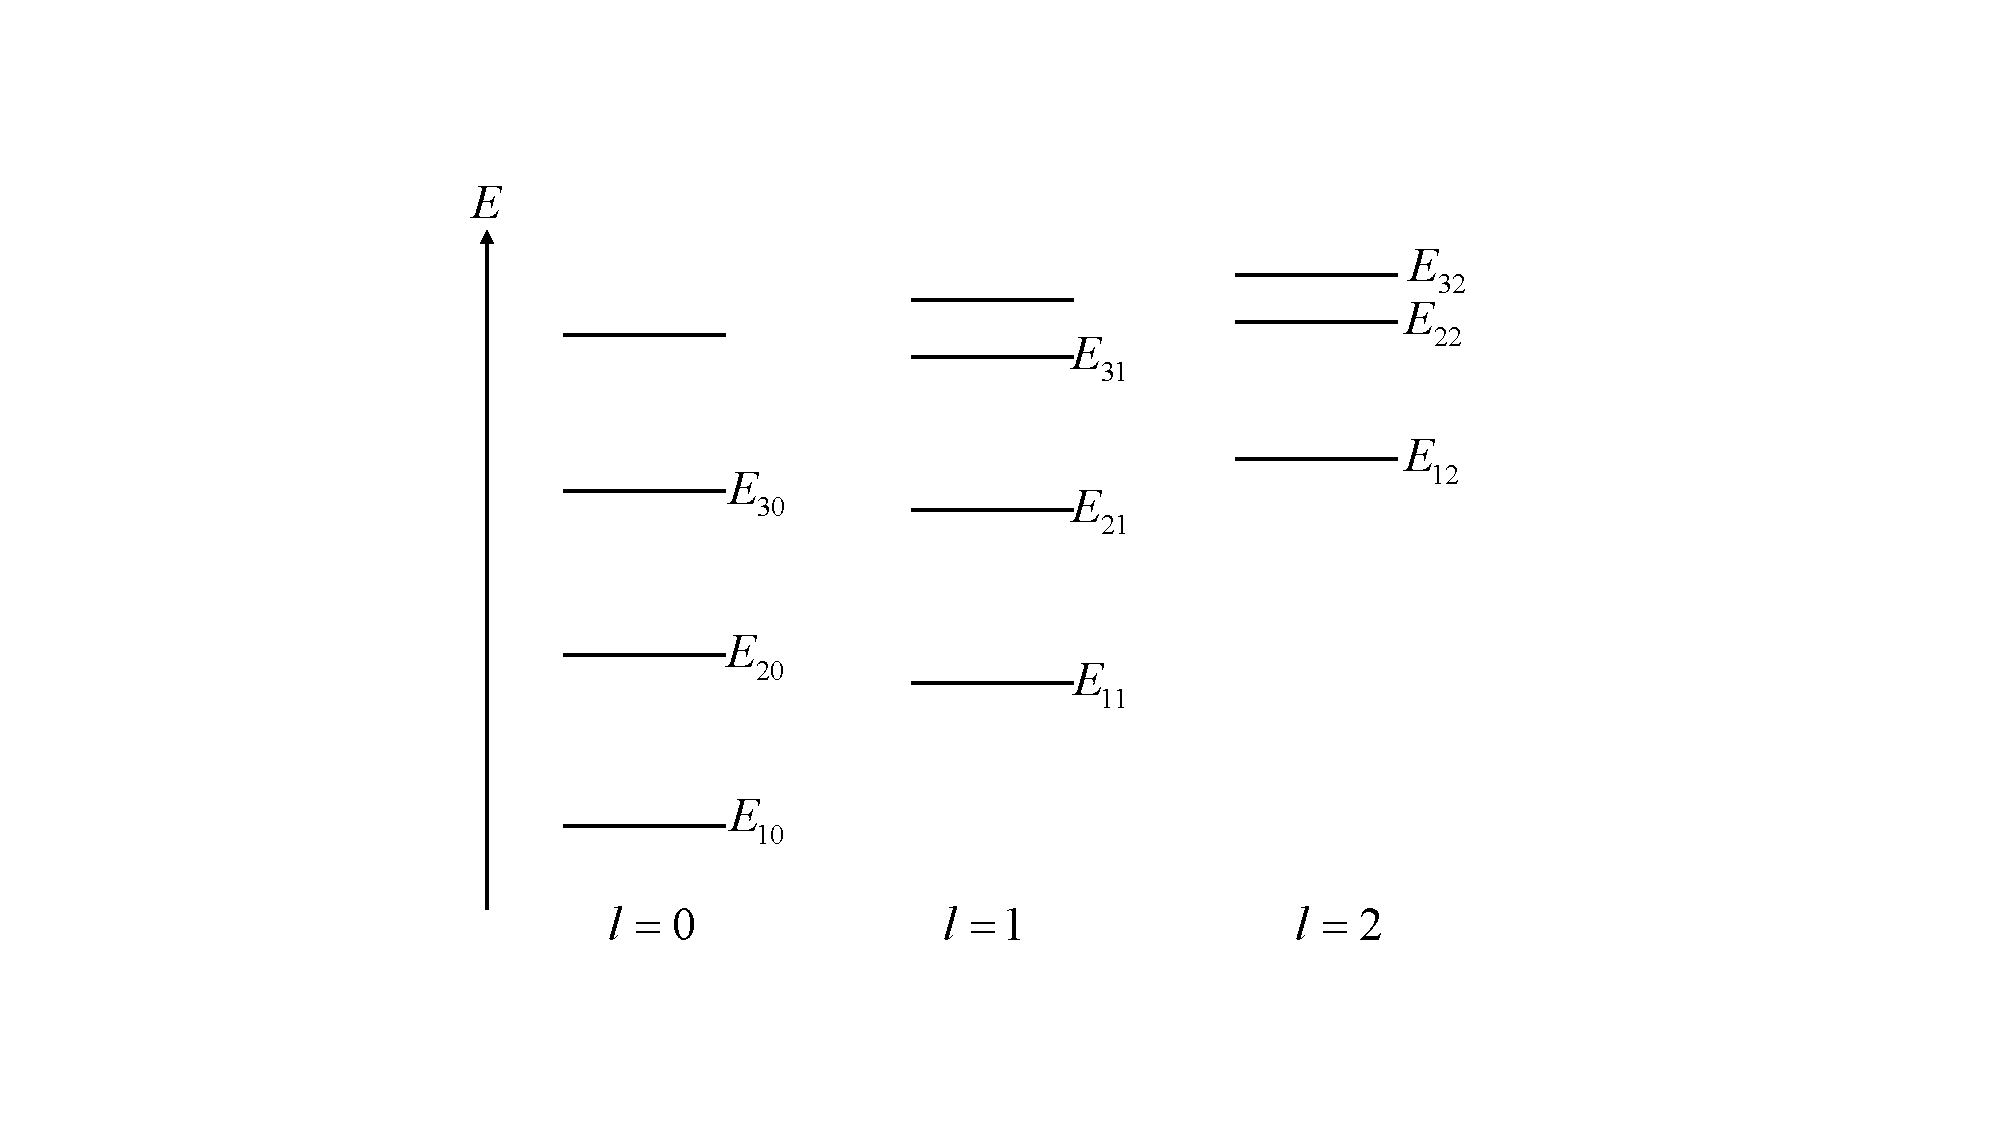
\includegraphics[width=6cm,clip]{QM file/figure/5-1}
	\caption{中心力场能级示意图}\label{fig.5-1}
\end{figure}

由于径向方程与$L_{z}$的量子数(磁量子数)$m$无关,因此能级$E_{nl}$($n=1,2,\cdots$为编号数)也与$m$无关.给定$l$后,$m$共有$(2l+1)$种取值,相应于$(2l+1)$种不同的状态[见\eqref{eq51.10}式],因此能级$E_{nl}$的简并度为$(2l+1)$.在具体问题中,属于不同$l$值的能级还可能出现重合,从而加大能级的简并度.氢原子和谐振子的能级都有这种“额外”的简并化.

{\heiti 4. 宇称性}

本征函数\eqref{eq51.10}式具有明确的宇称性.当$\boldsymbol{r}\rightarrow-\boldsymbol{r}$,$r$不变,$\theta\rightarrow\pi-\theta,\varphi\rightarrow\varphi+\pi$,径向波函数$R(r)$总是偶宇称,$Y_{lm}$的宇称则为$(-1)^{l}$,即
\begin{empheq}{equation}\label{eq51.23}
	Y_{lm}(\pi-\theta,\varphi+\pi)=(-1)^{l}Y_{lm}(\theta,\varphi)
\end{empheq}
这从\eqref{eq51.7}式及$P_{l}^{m}$的定义不难看出.因此\eqref{eq51.10}式的宇称为$(-1)^{l}$.属于相邻$l$的波函数宇称相反.基态属于$l=0$,为偶宇称.

{\heiti 5. 轨道磁矩}

\begin{wrapfigure}[14]{r}{4em}
	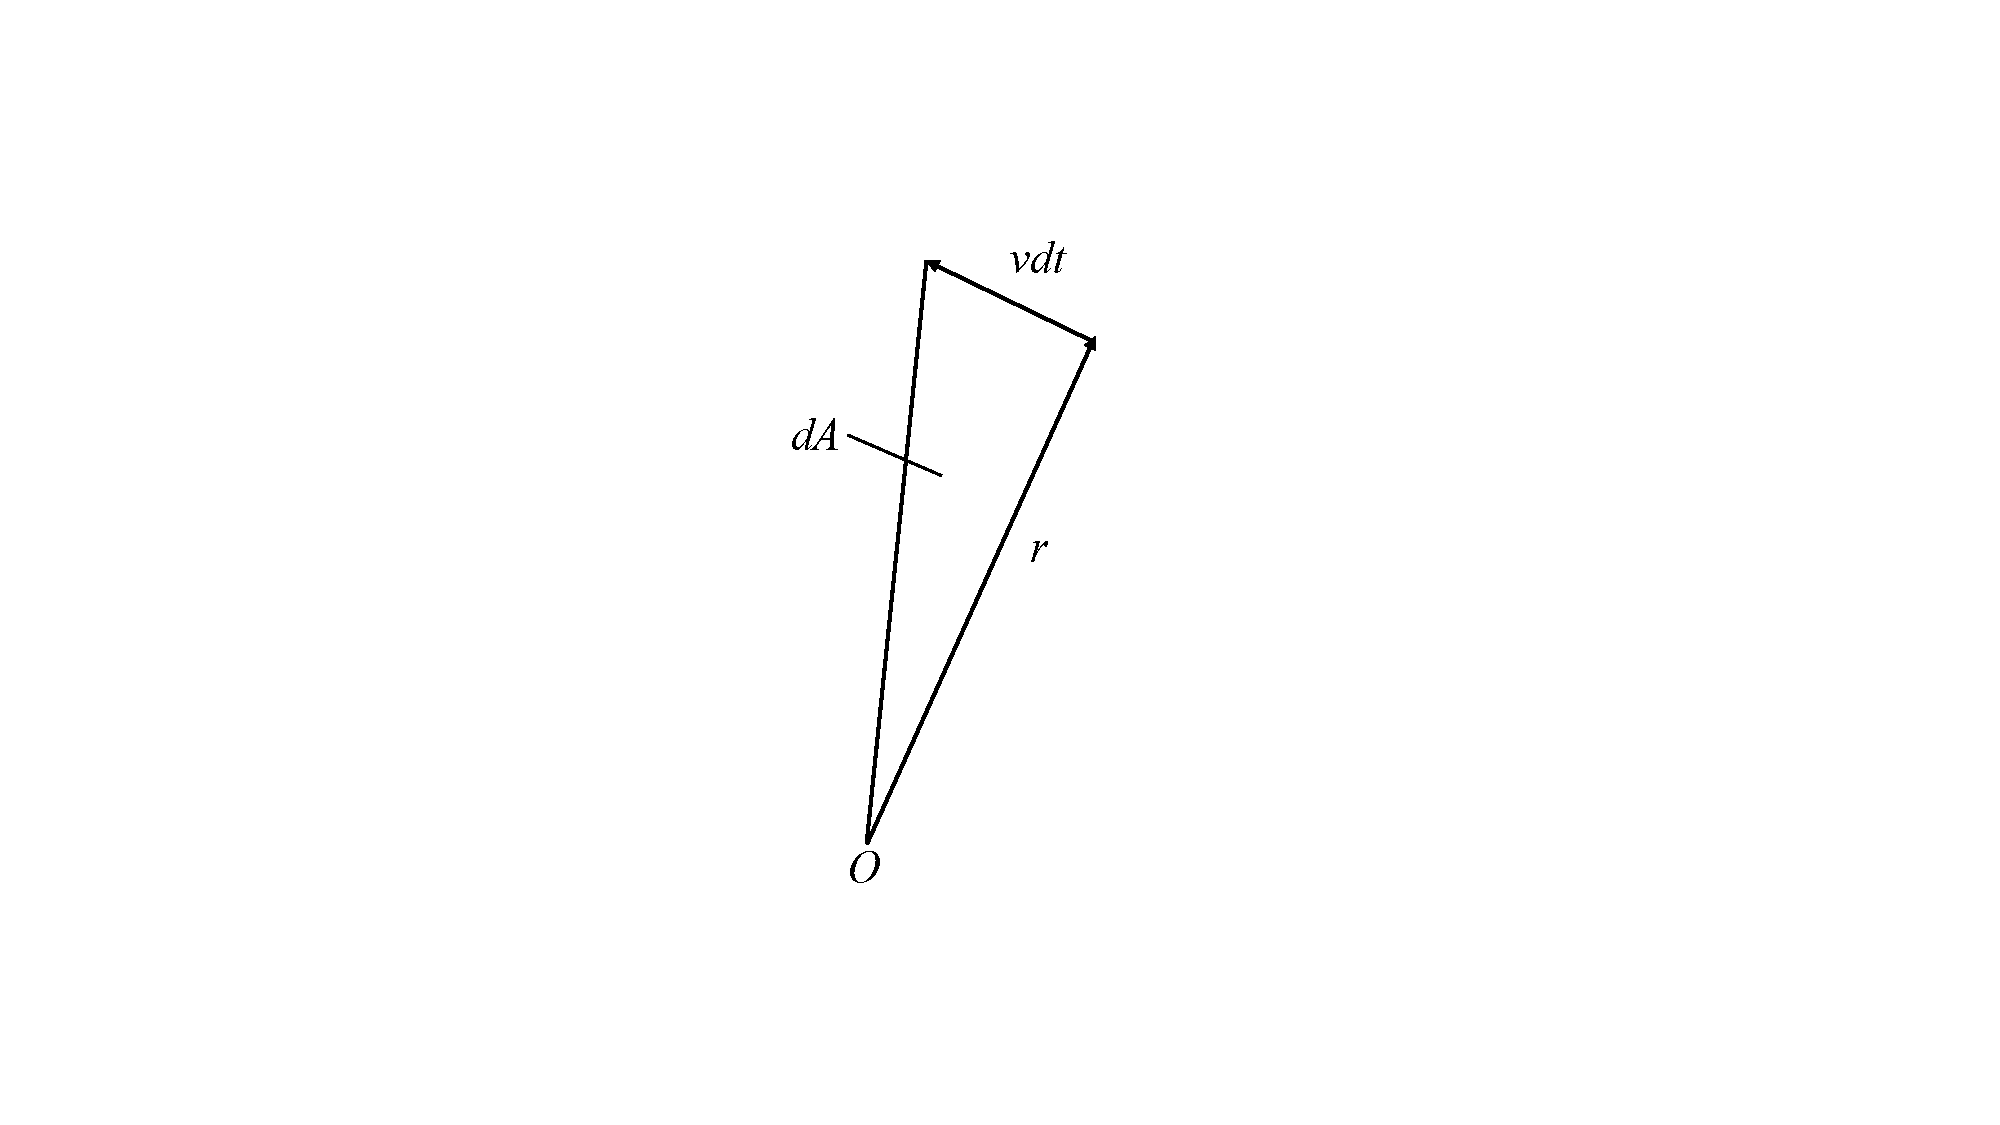
\includegraphics[width=2cm]{QM file/figure/5-2}
	\caption{}\label{fig.5-2}
\end{wrapfigure}
在经典力学中,质量为$\mu$电荷为$q$的粒子受中心力作用而沿平面闭合曲线作周期运动时,如图\ref{fig.5-2}所示,矢径$\boldsymbol{r}$的掠面速度为
\eqlong
\begin{empheq}{equation*}
	\frac{d\boldsymbol{A}}{dt}=\frac{1}{2}\boldsymbol{r}\times\boldsymbol{v}=\frac{1}{2\mu}\boldsymbol{r}\times\boldsymbol{p}=\frac{\boldsymbol{L}}{2\mu}
\end{empheq}
轨道曲线所围面积为
\begin{empheq}{equation}\label{eq51.24}
	\boldsymbol{A}=\oint d\boldsymbol{A}=\oint\frac{\boldsymbol{L}}{2\mu}dt=\frac{\tau}{2\mu}\boldsymbol{L}
\end{empheq}\eqnormal
其中$\boldsymbol{L}$为轨道角动量,$T$为周期.这种周期运动相当于一个环形电流回路,相应的等效电流为
\eqindent{9}
\begin{empheq}{equation}\label{eq51.25}
	I=\frac{q}{\tau}
\end{empheq}\eqnormal
等效磁矩为
\begin{empheq}{equation}\label{eq51.26}
	\boldsymbol{\mu}_{L}=\boldsymbol{IA}=\frac{q}{2\mu}\boldsymbol{L}\quad\text{国际单位制}
\end{empheq}
或
\begin{empheq}{equation*}\label{eq51.26'}
	\boldsymbol{\mu}_{L}=\frac{1}{c}\boldsymbol{IA}=\frac{q}{2\mu c}\boldsymbol{L}\quad\text{高斯单位制}	\tag{$5.1.26^{\prime}$}
\end{empheq}
在量子力学中,对于带电粒子的运动,轨道磁矩算符$\hat{\boldsymbol{\mu}}_{L}$就按\eqref{eq51.26}、\eqref{eq51.26'}式定义,其中$\boldsymbol{L}$理解为轨道角动量算符.当波函数为\eqref{eq51.10}式时,$L_{z}$取本征值$m\hbar$,$L_{x}$与$L_{y}$的平均值为0,因此$\boldsymbol{\mu}_{L}$的$z$分量取量子化的本征值:
\begin{empheq}{equation}\label{eq51.27}
	(\boldsymbol{\mu}_{L})_{z}=\frac{q\hbar}{2\mu}m\quad\text{国际单位制}
\end{empheq}
或
\begin{empheq}{equation*}\label{eq51.27'}
	(\boldsymbol{\mu}_{L})_{z}=\frac{q\hbar}{2\mu c}m\quad\text{高斯单位制}	\tag{$5.1.27^{\prime}$}
\end{empheq}
而$(\boldsymbol{\mu}_{L})_{x}$与$(\boldsymbol{\mu}_{L})_{y}$的平均值均等于零.

对于电子,电荷$q=-e$,质量$\mu=m_{e}$,如引入“玻尔磁子”:
\eqllong
\begin{empheq}{equation}\label{eq51.28}
	\mu_{B}=\frac{e\hbar}{2m_{e}}\quad\text{国际单位制},\quad\mu_{B}=\frac{e\hbar}{2m_{e}c}\text{高斯单位制}
\end{empheq}\eqnormal
则轨道磁矩的量子化本征值可以表示成
\begin{empheq}{equation}\label{eq51.29}
	(\boldsymbol{\mu}_{z})=-m\mu_{B},m=0,\pm1,\pm2,\cdots
\end{empheq}

{\heiti 6. 平均电流}

当粒子处于$\varPsi$态,$\S$\ref{sec:02.02}讲过的统计意义下的电流密度应该理解成平均电流密度,即
\begin{empheq}{equation}\label{eq51.30}
	j_{e}=-\frac{i\hbar}{2\mu}q(\varPsi^{*}\nabla\varPsi-\varPsi\nabla\varPsi^{*})
\end{empheq}
利用梯度算符的球坐标表示式[见附录\ref{A03}]
\begin{empheq}{equation}\label{eq51.31}
	\nabla=\boldsymbol{e}_{r}\frac{\partial}{\partial r}
	+\boldsymbol{e}_{\theta}\frac{1}{r}\frac{\partial}{\partial \theta}
	+\boldsymbol{e}_{\varphi}\frac{1}{r\sin\theta}\frac{\partial}{\partial \varphi}
\end{empheq}
$\boldsymbol{j}_{e}$可以表示成
\begin{empheq}{equation}\label{eq51.32}
	j_{e}=\boldsymbol{e}_{r}j_{r}+\boldsymbol{e}_{\theta}j_{\theta}+\boldsymbol{e}_{\varphi}j_{\varphi}
\end{empheq}
其中$\boldsymbol{e}_{r},\boldsymbol{e}_{\theta},\boldsymbol{e}_{\varphi}$中分别代表$\boldsymbol{r}$处沿半径方向、经线($\theta$增加方向)、纬线($\varphi$增加方向)方向的单位矢量,$j_{r},j_{\theta},j_{\varphi}$为$\boldsymbol{j}_{e}$在这三个方向的投影.即
\eqlong
\begin{empheq}{equation}\label{eq51.33}
	\begin{aligned}
		j_{e}&=-\frac{i\hbar}{2\mu}q(\varPsi^{*}\frac{\partial}{\partial r}\varPsi-\varPsi\frac{\partial}{\partial r}\varPsi^{*})	\\
		j_{\theta}&=-\frac{i\hbar}{2\mu}q\frac{1}{r}(\varPsi^{*}\frac{\partial}{\partial \theta}\varPsi-\varPsi\frac{\partial}{\partial \theta}\varPsi^{*})	\\
		j_{\varphi}&=-\frac{i\hbar}{2\mu}q\frac{1}{r\sin\theta}(\varPsi^{*}\frac{\partial}{\partial \varphi}\varPsi-\varPsi\frac{\partial}{\partial \varphi}\varPsi^{*})
	\end{aligned}
\end{empheq}
当波函数$\varPsi$为\eqref{eq51.10}式时,
\begin{empheq}{equation*}
	\varPsi(r,\theta,\varphi)=R(r)Y_{lm}(\theta,\varphi)=cR(R)P_{l}^{m}(\cos\theta)e^{im\varphi}
\end{empheq}\eqnormal
$\varPsi$中$\theta$部分$P_{l}^{m}(\cos\theta)$是实数,因此$j_{\theta}=0$.对于束缚态,径向波函数$R(r)$是实数,因此$j_{e}=0$.只有$j_{\varphi}\neq 0$中$\varphi$部分是$e^{im\varphi}$,因此
\begin{empheq}{equation*}
	\frac{\partial}{\partial \varphi}\varPsi=im\varphi,\quad \frac{\partial}{\partial \varphi}\varPsi^{*}=-im\varPsi^{*}
\end{empheq}\eqshort
\begin{empheq}{equation}\label{eq51.34}
	j_{\varphi}=\frac{\hbar q}{\mu}m\frac{\varPsi^{*}\varPsi}{r\sin\theta}
\end{empheq}\eqnormal
$j_{\varphi}$是$r,\theta$的函数,而与$\varphi$无关,平均电流沿各纬线流动,呈圆环状.早先安培曾假设原子中存在环状电流,现在得到了理论证明.如沿纬线取横截面元$rd\theta dr$,形成细圆环,其体积为
\eqlong
\begin{empheq}{equation}\label{eq51.35}
	d\tau=2\pi r\sin\theta\cdot rd\theta dr=2\pi r^{2}\sin\theta d\theta dr
\end{empheq}
环中平均电流为
\begin{empheq}{equation}\label{eq51.36}
	dI=j_{\varphi}rd\theta dr=\frac{\hbar q}{\mu}m\frac{\varPsi^{*}\varPsi}{\sin\theta}d\theta dr
\end{empheq}
$dI$对等效磁矩(平均值)的贡献为
\begin{empheq}{equation}\label{eq51.37}
	dM_{z}=\frac{1}{c}dI\cdot\pi(r\sin\theta)^{2}=m\frac{\hbar q}{2\mu c}\varPsi^{*}d\tau
\end{empheq}
各细电流环贡献的总等效磁矩(平均值)为
\begin{empheq}{equation}\label{eq51.38}
	M_{z}=\int dM_{z}=m\frac{\hbar q}{2\mu c}\int\varPsi^{*}\varPsi d\tau=m\frac{\hbar q}{2\mu c}
\end{empheq}\eqnormal
(高斯单位制)这正是\eqref{eq51.27'}式给出的轨道磁矩$(\boldsymbol{\mu}_{L})_{z}$的本征值.




